\documentclass[t]{beamer}
\usetheme{Warsaw}
\usecolortheme{seahorse}
\usepackage{array}
%\usepackage{graphicx}
\usepackage{amssymb,amsmath,mathrsfs,amsfonts}
%\usepackage[colorhighlight,display]{texpower}
%\usepackage{caption}
%\usepackage[all]{xy}
\usepackage{beamerthemesplit}
\mode<presentation>
%\usepackage{pause}
\usepackage{ulem}  % for strikethroughs
\usepackage{cancel} % for strikethroughs in math mode 
\usepackage{tikz}
\usepackage{calc}
\usetikzlibrary{shapes}
\usepackage{hyperref}
\hypersetup{pdfpagemode=FullScreen}
\usepackage{ifthen}
\usepackage{animate}
\usepackage{color}
\usepackage{type1cm}  % used for watermarking
\usepackage{eso-pic}  % used for watermarking


\theoremstyle{plain}
\newtheorem{prop}{Proposition}
\newtheorem{thm}[prop]{Theorem}
\newtheorem{lem}[prop]{Lemma}
\newtheorem{cor}[prop]{Corollary}
\theoremstyle{definition}
\newtheorem{dfn}{Definition}
\newtheorem{rem}[prop]{Remark}
\newtheorem{ex}{Example}[section]
%\newtheorem{note}{Note}[section]
\newtheorem{exercise}{Exercise}[section]
\newcommand{\nin}{\noindent}
\newcommand{\ds}{\displaystyle}
\renewcommand{\figurename}{Figure \arabic{figure}}



\renewcommand*\familydefault{\sfdefault} 




%%%%%%%%%%%%%%%%%%%%%%%%%%5
%%%%%%%%%%%%%%%%%%%%%%%%%%%%
%%%% some commands that have different meaning in the article/presentation modes

\newcommand{\vvfill}{\mode<presentation>{\vfill}  \mode<article>{\medskip}}   %vfill in presentation only
\newcommand{\sketchspace}{ 
\mode<article>{ \medskip\noindent{\textbf{Sketch:}} \vspace*{6cm} }
\mode<presentation>{ } 
}
\newcommand{\examplespace}{ 
\mode<article>{ \medskip\noindent{\textbf{Example:}} \vspace{6cm} }
\mode<presentation>{ } 
}
\newcommand{\artsmspace}{\mode<article>{\vspace*{2cm}} }  %small space in article mode
\newcommand{\artlargespace}{\mode<article>{\vspace*{6cm}} }  %large space in article mode

\newcommand{\dx}{\,dx}

\newcommand{\soln}{{\textbf{Solution: }}\,\,\,}
\newcommand{\disp}{\displaystyle}

\newcommand{\makedate}{\vvfill
\begin{picture}(10,10)  
\put(260,-20){\mbox{\tiny{\today}}}
\end{picture}
}

\newcommand{\pd}[2]{\dfrac{\partial#1}{\partial#2}}
\newcommand{\pD}[2]{\dfrac{\partial^2#1}{\partial#2^2}}
\newcommand{\pdd}[3]{\dfrac{\partial^2#1}{\partial#2 \partial#3}}


\normalem %stops the ulem package making all the emphs into underlines....
 
 
 
 \newcommand{\refandrev}[2]{
 \begin{small}
  \hspace{6cm}
  \begin{minipage}[r]{8cm}
  Stewart,    Chapter #1   \\
  Review:  \parbox[t]{6cm}{#2}
\end{minipage}
\end{small}
}



\newcounter{heading}
\setcounter{section}{1}
\setcounter{heading}{0}

\newcommand{\makeheading}[1]{\medskip\begin{large}\noindent\textbf{{#1}}\end{large}\smallskip}

%\newenvironment{head}[1]{\medskip\stepcounter{heading}\noindent\textbf{\hspace{0.2cm}{#1}.}}{}
\newcommand{\newhead}[1]{\medskip\stepcounter{heading}\noindent\textbf{\hspace{0.2cm}{#1}.}}


\newcommand{\pf}[1]{\noindent\textit{Proof.}\vspace*{#1 cm}}
\newcommand{\sol}[1]{\noindent\textit{Solution.}\vspace*{#1 cm}}
\newcommand{\further}[1]{\begin{small}\noindent\textit{Further reading: #1}\end{small}}
\newcommand{\exr}[1]{\begin{footnotesize}\noindent\textit{\textbf{Exercises:} Stewart #1}\end{footnotesize}}


% Sets of numbers
\newcommand{\C}{\mathbb{C}}
\newcommand{\RR}{\mathbb{R}}
\newcommand{\Z}{\mathbb{Z}}
\newcommand{\N}{\mathbb{N}}
\newcommand{\Q}{\mathbb{Q}}

% Partitions
\newcommand{\PP}{\mathcal{P}}

% Limits
\newcommand{\limm}[1]{\displaystyle \lim_{x\to #1}}

% Backslash
\newcommand{\bs}{\backslash}

% functions
\newcommand{\cosec}{\mathrm{cosec}}
\newcommand{\cosech}{\mathrm{cosech}}
\newcommand{\sech}{\mathrm{sech}}
\newcommand{\Li}{\mathrm{Li}}
\newcommand{\si}{\mathrm{Si}}
\newcommand{\erf}{\mathrm{erf}}

% Domain and Range
\newcommand{\Dom}{\mathrm{Dom}}
\newcommand{\Codom}{\mathrm{Codom}}
\newcommand{\Range}{\mathrm{Ran}}



\title{Week 7:  Fundamental Theorem of Calculus}
%\date{September 3 -- September 7, 2012}

\begin{document}

\frame{\titlepage}

\setcounter{tocdepth}{2}
\frame{\tableofcontents

}

\AtBeginSection[]
{
\begin{frame}<beamer> 
\tableofcontents[currentsection]  % show TOC and highlight current section
\end{frame}
}


\section{Fundamental Theorem of Calculus}

\begin{frame}
\begin{theorem}[Fundamental Theorem of Calculus]
Suppose a function $f$ is continuous on $[a,b]$, then
\begin{enumerate}
\item $g(x)=\ds\int^x_af(t)\,dt$ for $x\in [a,b]$, and $g'(x)=f(x)$
\item $\ds\int_a^bf(x)\dx=F(b)-F(a)$
\begin{itemize}
	\item where $F$ is an antiderivative of $f$,  i.e., $F' = f$
	\item Other common notation is $F(x)\big]_{a}^{b}= F(b) - F(a)$
\end{itemize}
\end{enumerate}
\end{theorem}

\begin{figure}
\begin{center}
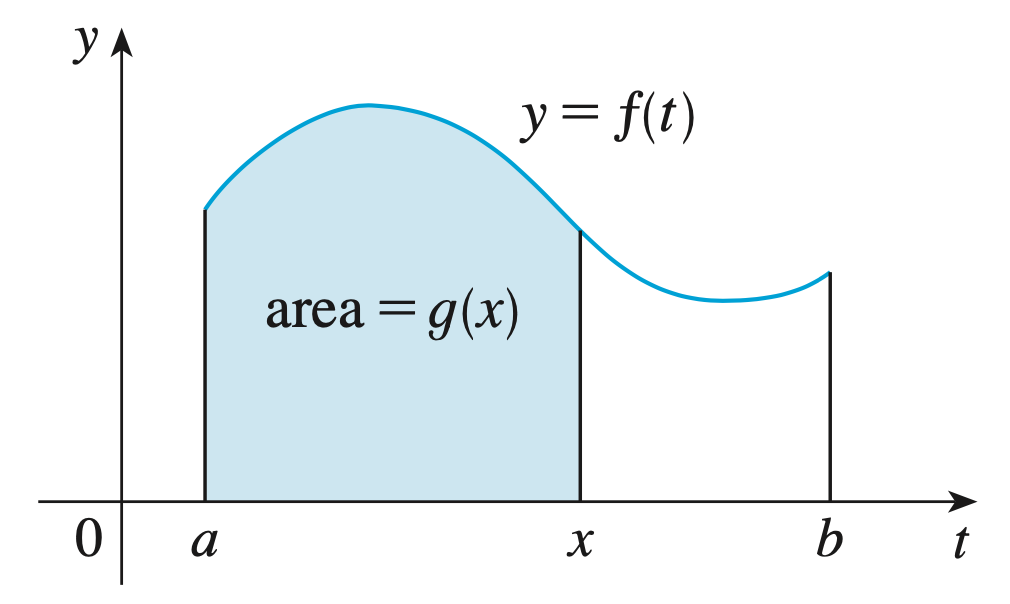
\includegraphics[scale=0.27]{fig/ftc0}
\end{center}
\end{figure}

\end{frame}

\subsection{Part 1}

\begin{frame}

\frametitle{Why}

\begin{figure}
\begin{center}
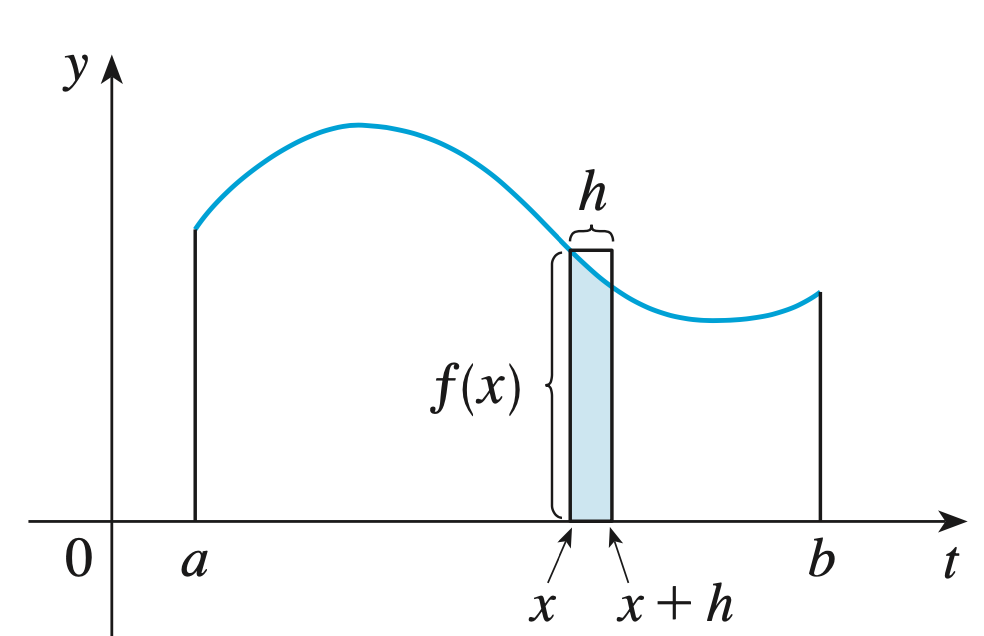
\includegraphics[scale=0.27]{fig/ftc1}
\end{center}
\end{figure}

\begin{itemize}
%\item $g(x)=\ds\int^x_af(t)\,dt$\\
\item $g(x + h) - g(x) \approx h \cdot f(x)$\\
\item $\dfrac{g(x+h)-g(x)}{h} \approx f(x)$
\item $g'(x) = \ds\lim_{h\rightarrow 0} \dfrac{g(x+h)-g(x)}{h} = f(x)$ 
\item Thus, $g' = f$
\end{itemize}

\end{frame}

\begin{frame}

\frametitle{Example}

\footnotesize

Find these derivatives using Theorem Part 1.

%$$g(x)=\ds\int^x_af(t)\,dt \text{ for } x \text{ in } [a,b],  g'(x)=f(x) \text{ for all } x\text{ in } (a,b)$$

\begin{enumerate}
	\item $\dfrac{d}{dx} \ds\int_{5}^x \sqrt{t^2 + 3}\, dt = \sqrt{x^2 + 3}$
	\item $\dfrac{d}{dx} \ds\int_{4}^x \sqrt{t^2 + 3}\, dt = \sqrt{x^2 + 3}$
	\item $\dfrac{d}{dx} \ds\int_{x}^4 \sqrt{t^2 + 3}\, dt = \dfrac{d}{dx} \left(-\ds\int_{4}^x \sqrt{t^2 + 3}\, dt \right)= -\sqrt{x^2 + 3}$
	\item $\dfrac{d}{dx} \ds\int_{4}^{\sin{x}} \sqrt{t^2 + 3}\, dt$
	\begin{itemize}
		\item Let $u$ be $\sin{x}$
		\item $\dfrac{d}{dx} \ds\int_{4}^{\sin{x}} \sqrt{t^2 + 3}\, dt = \dfrac{d}{du} \ds\int_{4}^{u} \sqrt{t^2 + 3}\, dt \cdot \dfrac{du}{dx} = \sqrt{u^2 + 3}\cdot \cos{x} = \sqrt{(\sin{x})^2 + 3}\cdot \cos{x}$
	\end{itemize}
\end{enumerate}

\end{frame}

\begin{frame}

\frametitle{Exercise}

\footnotesize

Find these derivatives using Theorem Part 1.

\begin{itemize}
	\item $\dfrac{d}{dx} \ds\int_{0}^{x} \sqrt{t + t^3} \,dt $
	\begin{itemize}
		\item Ans: $\sqrt{x + x^3}$
	\end{itemize}
	\item $\dfrac{d}{dx} \ds\int_{1}^{x^4} \sec{t} \,dt $
	\begin{itemize}
		\item Ans: $\sec{x^4} \cdot 4x^3$
	\end{itemize}
	\item $\dfrac{d}{dx} \ds\int_{1}^{e^x} \ln{t} \,dt $
	\begin{itemize}
		\item $ \ln{e^x} \cdot  e^x = xe^x$
%		\item Let $u$ be $e^x$
%		\item $\dfrac{d}{dx} \ds\int_{1}^{e^x} \ln{t} \,dt  = \dfrac{d}{du} \ds\int_{1}^{u} \ln{t} \, dt \cdot \dfrac{du}{dx}  = \ln{u} \cdot  \dfrac{du}{dx} =
	\end{itemize}
\end{itemize}

\end{frame}

\subsection{Part 2}

\begin{frame}

\frametitle{Example}

Recall the part 2 theorem as follows:

\medskip

If $F$ is an antiderivative of $f$, then \[ \int_a^bf(x)\dx= F(x)\big]_{a}^{b} = F(b)-F(a)\] 

Evaluate the integral $\ds\int_{1}^{3} e^x \,dx$ \pause

\begin{itemize}
	\item $F = e^x$
	\item $F(3) - F(1)$
	\item $e^3 - e$
\end{itemize}

\end{frame}

\begin{frame}

\frametitle{Example}

Evaluate the integral $\ds\int_{0}^{1} x^2 \,dx$ \pause

\begin{itemize}
	\item $F = \dfrac{x^3}{3}$
	\item $F(1) - F(0)$
	\item $\dfrac{1^3}{3} - \dfrac{0^3}{3} = \dfrac{1}{3}$
\end{itemize}

\end{frame}
%
%\begin{frame}
%
%\frametitle{Example}
%
%Evaluate the integral $\ds\int_{3}^{6} \dfrac{1}{x} \,dx$ \pause
%
%\begin{itemize}
%	\item $F = \ln{x}$
%	\item $F(6) - F(3)$
%	\item $\ln{6} - \ln{3} = \ln{\dfrac{6}{3}} = \ln{2}$
%\end{itemize}
%
%\end{frame}
%
%\begin{frame}
%
%\frametitle{Example}
%
%Evaluate the integral $\ds\int_{0}^{\frac{\pi}{2}} \cos{x} \,dx$ \pause
%
%\begin{itemize}
%	\item $F = \sin{x}$
%	\item $F(\frac{\pi}{2}) - F(0)$
%	\item $\sin{\frac{\pi}{2}} - \sin{0} = 1 - 0 = 0$
%\end{itemize}
%
%\end{frame}
%
\begin{frame}

\frametitle{Example (caution!)}

Evaluate the integral $\ds\int_{-1}^{3} \dfrac{1}{x^2} \,dx$ \pause
 
 \begin{itemize}
	\item $F = \dfrac{-1}{x}$
	\item $F(3) - F(-1)$
	\item $\dfrac{-1}{3} - \dfrac{-1}{-1} = \dfrac{-1}{3} - 1 = \dfrac{-4}{3}$
\end{itemize}

\medskip

This violates the comparison property, recall this property:  $$\text{If } f(x)\geq0 \text{ for all } x \text{ in } [a,b] \text{ then } \int_a^b f(x)\,dx\geq0$$

Looking more deeply, $f(x) = \dfrac{1}{x^2}$ has an infinite discontinuity at $x = 0$, thus the integral does not exist.

\end{frame}

\begin{frame}

\frametitle{Exercise}
 
 \begin{itemize}
	\item  $\ds\int_{1}^{3} (x^2 + 2x -4) \,dx$
	\begin{itemize}
		\item Ans: $\frac{26}{3}$
	\end{itemize}
	\item $\ds\int_{0}^{4} (4-t)\cdot \sqrt{t} \,dt$
	\begin{itemize}
		\item Ans: $\frac{128}{15}$
	\end{itemize}
	\item $\ds\int_{0}^{3} (2\sin{x} - e^x) \,dx$
	\begin{itemize}
		\item Ans: $3 - 2\cos{3} - e^3$
	\end{itemize}
	\item $\ds\int_{-2}^{2} f(x) = \begin{cases}
       2 & \text{if } -2 \leq x \leq 0\\
       4 - x^2 & \text{if } 0 < x \leq 2\\
        \end{cases}$
	\begin{itemize}
		\item Ans: $\dfrac{28}{3}$
	\end{itemize}
\end{itemize}

\end{frame}
%
%\begin{frame}
%\newhead{Remarks on Part 1}
%\begin{itemize}
%\item[(a)] Part 1 tells us that \emph{every} function defined by an integral is differentiable, and  $g'(x) = f(x)$.
%\item[(b)]  Also, \textit{every} continuous function $f$ on $(a,b)$ has an antiderivative $g$, where $g$ is defined as the integral of $f$ from $a$ to $x$.
%\end{itemize}
%\newhead{Examples}  Find the derivative of $g$, where $g$ is given by
%\begin{enumerate}
%\item[(i)] $g(x) = \int_{0}^{x}\sqrt{1 + t^{2}}\,dt.$
%\vspace*{.3cm}
%\item[(ii)] $g(x) = \int_{5}^{x}\sqrt{1 + t^{2}}\, dt.$
%\vspace*{.3cm}
%\item[(iii)] $g(x) = \int_{3}^{17}\sqrt{1+t^{2}}\,dt.$
%\end{enumerate}
%\end{frame}
%
%\begin{frame}
%\newhead{Remarks on Part 2}
%\begin{enumerate}
%\item[(a)] Note that the left hand side of the above equation is found by taking the limit of Riemann sums, which involves knowing the value of $f$ at \textbf{all} points between $a$ and $b$.  The right hand side, however, only requires knowing the value of $F$ at \textbf{two} points!
%
%\item[(b)] A common misconception is that this formula is the \emph{definition} of the definite integral.  It is not, the definition of integral is the limit of Riemann sums.  
%
%\item[(c)] We use the notation $F(x)\big|_{a}^{b} = F(b) - F(a)$.  Another common notation is $F(x)\big]_{a}^{b}$, which is used in the book.
%\item[(d)] When we apply the FTC, part 2, we may use \emph{any} antiderivative of $f$ (recall that if $F' = f$, the most general form for an antiderivative of $f$ is $F + C$, where $C$ is an arbitrary constant).
%\end{enumerate}
%\end{frame}
%
%\begin{frame}
%\newhead{Remarks on Part 2}
%\begin{enumerate}
%\item[(e)] The FTC, part 2 is quite plausible from a physical perspective.  Recall that when we considered the ``Distance Problem'' several lectures ago, we determined that the area under the velocity curve was equal to the total distance travelled.  That is, if velocity and position are given by $v(t)$ and $s(t)$ respectively at time $t$, then $s'(t) = v(t)$, so $s$ is an antiderivative of $v$, and $\int_{a}^{b}v(t)\, dt = s(b) - s(a)$.
%\end{enumerate}
%\end{frame}

\subsection{Indefinite Integral}

\begin{frame}

\begin{dfn} If $F'(x) = f(x)$, we write $\int f(x)\, dx = F(x)+C$ and call the symbol $\int f(x)\, dx$ the \textbf{indefinite integral} of $f$, and $C$ is called the \textbf{constant of integration}.\end{dfn}

\medskip

\noindent Note that the \textbf{definite} integral is a \emph{number}, whereas the \textbf{indefinite} integral is a \emph{function}, or a \emph{family of functions}. 

\medskip

Example: $\ds\int (10x^4 - 2\sec{x}^2) \, dx = 10\cdot \dfrac{x^5}{5} - 2 \tan{x} + C = 2x^5 - 2 \tan{x} + C$

\end{frame}

%
%\begin{frame}
%\newhead{A table of indefinite integrals}\\
%In the following table, $c, C,$ and $k$ are arbitrary constants.
%
%\begin{center}
%\renewcommand{\arraystretch}{1.5}
%\begin{tabular}{| c | c |}
%\hline
%$f$ & $\int f(x)\,dx$ \\
%\hline
%$cf(x)$ & $c(\int f(x)\,dx)+C$ \\
%$f(x)\pm g(x)$ & $(\int f(x)\,dx) \pm (\int g(x)\,dx) +C$ \\
%$k$ & $kx + C$ \\
%$x^n$ (where $n\neq-1$) & $\ds\frac{x^{n+1}}{n+1}+C$ \\
%$\cos x$ & $\sin x+C$ \\
%$\sin x$ & $-\cos x+C$ \\
%$\sec^2 x$ & $\tan x+C$ \\
%$\sec x\,\tan x$ & $\sec x + C$ \\
%\hline
%\end{tabular}
%\end{center}
%\end{frame}
%
%\begin{frame}
%\newhead{Examples}
%\noindent Evaluate the following integrals:
%\begin{enumerate}
%\item [(i)] $\int_{\pi}^{2\pi} \cos \theta \, d\theta$
%\vspace*{.2cm}
%\item[(ii)] $\int_{0}^{1}x(\sqrt[3]{x} + \sqrt[4]{x})\,dx$
%\vspace*{.2cm}
%\item[(iii)] True or False:
%$\int_{0}^{\pi} \sec^{2}x\,dx = \tan x\big|_{0}^{\pi} = 0.$
%\vspace*{.2cm}
%\item[(iv)] Find the indefinite integral: $\int (1-t)(2+t^{2}) \, dt$.
%\end{enumerate}
%\end{frame}

\section{Substitution Rule}

\begin{frame}
\frametitle{Substitution Rule}
\begin{block}{The substitution rule}
If $u = g(x)$ is a differentiable function whose range is an interval $I$ and $f$ is continuous on $I$, then
\[ \int f(g(x))g'(x)\,dx = \int f(u)\,du.\]
That is, \emph{it is permissible to work with $dx$ and $du$ after integral signs as if they are differentials}.
\end{block}

\end{frame}

\begin{frame}

\frametitle{Example}

Find $\ds \int 2x \sin{x^2} \,dx $ \pause

\medskip

Let $u = x^2$ and $du = 2x \, dx$

\medskip

Thus,  $\ds \int \sin{u} \,du  =  -\cos{u} + C = -\cos{x^2} + C$

\end{frame}

\begin{frame}

\frametitle{Example}

Find $\ds \int \dfrac{x}{1 + 3x^2} \,dx $ \pause

\medskip

Let $u = 1 + 3x^2$ and $du = 6x \, dx$ or $\frac{1}{6} du = x \, dx$

\medskip

Thus,  $\ds \int \dfrac{x}{1 + 3x^2} \,dx  = \ds \int \dfrac{\frac{1}{6}}{u} \,du  = \dfrac{1}{6} \int \dfrac{1}{u} \, du$

\medskip

The antiderivative is $\dfrac{1}{6} (\ln{|u|} + C) = \dfrac{1}{6} (\ln{|1 + 3x^2|} + C)$

\end{frame}

\begin{frame}

\frametitle{Example}

Find $\ds \int e^{7x} \,dx $ \pause

\medskip

Let $u = 7x$ and $du = 7 \, dx$ or $\frac{1}{7}du = dx$

\medskip

Thus,   $\ds \int e^{u} \cdot \frac{1}{7} \,du  = \frac{1}{7} e^{u} + C =  \frac{1}{7} e^{7x} + C$

\end{frame}

\begin{frame}

\frametitle{Example}

\footnotesize

Find $\ds \int \sqrt{1 + x^2} \cdot x^5 \,dx $ \pause

\medskip

Let $u = 1 + x^2$ and $du = 2x \, dx$ so $x \, dx = \dfrac{1}{2} \,du$.  Also, $x^2 = u - 1$, so $x^4 = (u-1)^2$

\begin{align*}
\ds \int \sqrt{1 + x^2} \cdot x^5 \,dx &= \ds \int \sqrt{1 + x^2} \cdot x^4 \cdot x \,dx\\
&= \int \sqrt{u} \cdot (u-1)^2 \cdot \frac{1}{2} \,du\\
& = \frac{1}{2} \int \sqrt{u} (u^2 - 2u + 1) \, du \\
& = \frac{1}{2} \int (u^{\frac{5}{2}} - 2u^{\frac{3}{2}} + u^{\frac{1}{2}}) \, du\\
& = \frac{1}{2} (\frac{2}{7}u^{\frac{7}{2}} - 2 \cdot \frac{2}{5}u^{\frac{5}{2}} + \frac{2}{3}u^{\frac{3}{2}}) + C\\
& = \frac{1}{7}(1+x^2)^{\frac{7}{2}} - \frac{2}{5}(1+x^2)^{\frac{5}{2}} + \frac{1}{3}(1+x^2)^{\frac{3}{2}} + C
\end{align*}

\end{frame}

\begin{frame}

\frametitle{Example}

Find $\ds \int_{0}^{4} \sqrt{2x + 1} \, dx$ \pause

\medskip

Let $u =2x + 1$ and $dx =\frac{1}{2}\, du$ 

\medskip

Next, we need to change the bound of $x$ to $u$, i.e., when $x = 0, u = 2(0) + 1 = 1$; when $x = 4, u = 2(4) + 1 = 9$

\begin{align*}
\ds \int_{0}^{4} \sqrt{2x + 1} \, dx &= \int_{1}^{9} \frac{1}{2}\sqrt{u} \,du\\
&= \frac{1}{2} \cdot \frac{2}{3}u^{\frac{3}{2}} \ds\big]_{1}^{9}\\
&= \frac{1}{3} (9^{\frac{3}{2}} - 1^{\frac{3}{2}})\\
&= \frac{26}{3}
\end{align*}

\end{frame}



\begin{frame}

\frametitle{Exercise}

\begin{itemize}
	\item $\ds \int \tan{x} \,dx$
	\begin{itemize}
		\item $- \ln{|\cos{x}|} + C$
	\end{itemize}
	\item $\ds \int x^3 \cos({x^4 + 2})\,dx$
	\begin{itemize}
		\item $\frac{1}{4} \sin({x^4 + 2}) + C$
	\end{itemize}
	\item $\ds \int \sqrt{2x + 1} \, dx$
	\begin{itemize}
		\item $\frac{1}{3}(2x + 1)^{\frac{3}{2}} + C$
	\end{itemize}
	\item $\ds \int_{1}^{2} \dfrac{1}{(3 - 5x)^2} \, dx$
	\begin{itemize}
		\item $1/14$
	\end{itemize}
	\item $\ds \int_{1}^{e} \dfrac{\ln{x}}{x} \, dx$
	\begin{itemize}
		\item $1/2$
	\end{itemize}
\end{itemize}

\end{frame}



\end{document}